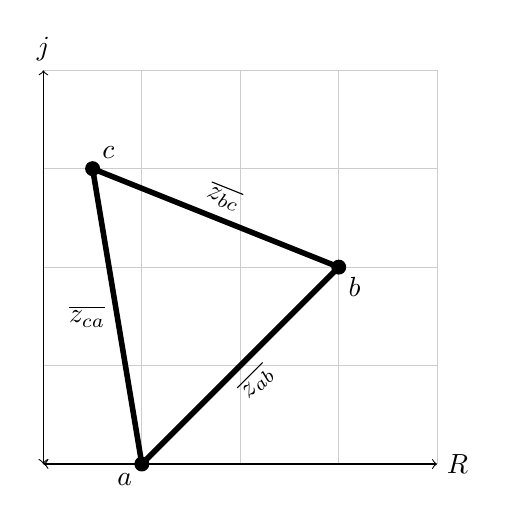
\begin{tikzpicture}[scale=1.25]
    \draw[thin,gray!40] (0,0) grid (4,4);
    \draw[<->] (0,0)--(4,0) node[right] {$R$};
    \draw[<->] (0,0)--(0,4) node[above]{$j$};
    \coordinate (a) at (1,0);
    \coordinate (b) at (3,2);
    \coordinate (c) at (0.5,3);
    
    \draw[fill=black] (a) circle(2pt) node[anchor=north east]{$a$};
    \draw[fill=black] (b) circle(2pt) node[anchor=north west]{$b$};
    \draw[fill=black] (c) circle(2pt) node[anchor=south west]{$c$};
    
    \draw[line width=2pt,black,-] (a)--(b) node[midway, below, sloped]{$\overline{z_{ab}}$};
    \draw[line width=2pt,black,-] (b)--(c) node[midway, above, sloped ]{$\overline{z_{bc}}$};
    \draw[line width=2pt,black,-] (c)--(a) node[midway, left]{$\overline{z_{ca}}$};
    
\end{tikzpicture}
\caption{Triangulo en el plano complejo con rectas parametrizadas}